% !TeX root = ../../libro.tex
% !TeX encoding = utf8

\chapter{Herramientas matemáticas fundamentales} \label{ch:matematicas_fundamentales}

En esta sección vamos a introducir algunas de las herramientas matemáticas sobre las que se apoya nuestro trabajo.

\section{Notación}

Seguiremos en parte la notación del \textit{paper} de referencia \cite{matematicas:principal}, aunque introducimos varios cambios por claridad, para no confundir en las fórmulas escalares, vectores y tensores.

Denotaremos a los vectores con flechas sobre las letras que los identifican, tal que $\nv{v} \in \R^N$. Las coordenadas de dicho vector se denotarán como $\nv{v_i}$ con $i \in \deltaset{n}$, donde $\deltaset{n} := \{1, \ldots, n\}$. También usaremos la notación $\doubledeltaset{n}{m} := \{n, \ldots, m\}$ donde $n \leq m$. En algunas ocasiones usaremos la notación $\nv{v_i^n}$ para indicar que estamos trabajando con el índice $i$ del vector $n$-ésimo de un conjunto de vectores.

Aunque más tarde definiremos qué significan estos conceptos, introducimos ahora la notación usada respecto a los tensores. Para denotar a los tensores usaremos tipografía caligráfica, por ejemplo, $\mathcal{A} \in \R^{M_1 \times \ldots \times M_N}$. Cada una de las entradas de dicho tensor serán denotadas como $\mathcal{A}_{d_1, \ldots, d_N} \in \R$. Al espacio de tensores de orden $N$ y dimensión $M$ en cada modo lo denotaremos por $\espaciotensores{N}{M}$. Al producto tensorial entre dos tensores $\mathcal{A}, \mathcal{B}$ lo denotaremos como $\mathcal{A} \otimes \mathcal{B}$. Dado un conjunto de vectores $\nv{v_1}, \ldots, \nv{v_N} \in \R^{M_1}, \ldots, \R^{M_N}$, denotaremos su producto tensorial $\nv{v_1} \otimes \cdots \otimes \nv{v_N}$ como $\otimes_{i = 1}^N \nv{v_i}$.

Por otro lado, al espacio de matrices de dimensiones $p, q$ lo denotaremos de la forma usual como  $\espaciomatrices{p}{q}$. Al producto de Kronecker entre dos matrices $A, B$ lo denotaremos como $A \odot B$.

\section{Tensores}

\subsection{Definición del producto tensorial} \label{sec:deftensor}

Dados dos espacios vectoriales reales \footnote{Podría realizarse la construcción sobre otro cuerpo.} $\mathbb{V}, \mathbb{W}$, queremos construir el espacio producto tensorial de estos espacios vectoriales, denotado como $\mathbb{V} \otimes \mathbb{W}$. Buscamos que este nuevo objeto matemático tenga propiedades similares a las del producto entre escalares, principalmente la propiedad distributiva y la propiedad asociativa.

Realizamos la construcción de este objeto en varios pasos. En primer lugar definimos el producto formal entre dos espacios vectoriales. Introducimos las propiedades que queremos que el producto formal cumpla y en base a esto definimos el producto tensorial. Finalmente, estudiamos algunas de las propiedades que tiene este nuevo objeto matemático.

\subsubsection{Producto formal de dos espacios vectoriales}

Para la construcción del producto tensorial de espacios vectoriales necesitaremos primero introducir el concepto de producto formal entre dos espacios vectoriales, que será fundamental en la construcción del objeto matemático que buscamos.

\begin{definicion}[Producto formal de dos espacios vectoriales]
	Sean $\mathbb{V}, \mathbb{W}$ dos espacios vectoriales reales. Se define su \textbf{producto formal} como:

	\begin{equation}
		\mathbb{V} \ast \mathbb{W} := \spanset{v \ast w : \; v \in \mathbb{V}, \; w \in \mathbb{W}}
	\end{equation}

	donde $*$ es un símbolo con el que no sabemos operar. Por tanto, ahora mismo no sabemos simplificar muchas expresiones en este espacio.
\end{definicion}

\begin{observacion}
	$\text{span}$ denota el conjunto formado por todas las combinaciones lineales finitas de los elementos del conjunto, es decir,

	\begin{equation}
		\spanset{A} := \{ \sum_{k = 1}^n \alpha_i a_i : \; n \in \N, \; \alpha_i \in \R, \; a_i \in A \}
	\end{equation}
\end{observacion}

Es claro que por ser $\mathbb{V}, \mathbb{W}$ espacios vectoriales, y estar tomando combinaciones lineales finitas, $\mathbb{V} \ast \mathbb{W}$ es un espacio vectorial.

\subsubsection{Producto tensorial a partir del producto formal} \label{sec:cociente_prod_formal}

Para motivar el nuevo objeto que vamos a construir, hay que tener en cuenta que en general las siguientes igualdades no se cumplen:

\begin{enumerate}
	\item $c [\nv{v} \ast \nv{w}] = (c\nv{v}) \ast \nv{w}$.
	\item $c[\nv{v} \ast \nv{w}] = \nv{v} \ast (c\nv{w})$.
	\item $(\nv{v_1} + \nv{v_2}) \ast \nv{w} = \nv{v_1} \ast \nv{w} + \nv{v_2} \ast \nv{w}$.
	\item $\nv{v} \ast (\nv{w_1} + \nv{w_2}) = \nv{v} \ast \nv{w_1} + \nv{v} \ast \nv{w_2}$.
\end{enumerate}

Donde estamos tomando $\nv{v}, \nv{v_1}, \nv{v_2} \in \mathbb{V}$, $\nv{w}, \nv{w_1}, \nv{w_2} \in \mathbb{W}, c \in \R$. Estas igualdades representan las propiedades que queremos que se cumplan para que nuestro nuevo objeto matemático tenga el comportamiento deseado. Como $\mathbb{V} \ast \mathbb{W}$ es un espacio vectorial, podemos usar el espacio cociente para introducir dichas propiedades. Para ello definimos:

\begin{equation}
	\begin{split}
		I := \spanset{ &
			(c\nv{v}) \ast \nv{w} - c(\nv{v} \ast \nv{w}), \nv{v} \ast (c\nv{w}) - c(\nv{v} \ast \nv{w}), (\nv{v_1} + \nv{v_2}) \ast \nv{w} - (\nv{v_1} \ast \nv{w} + \nv{v_2} \ast \nv{w}), \\
			& \nv{v} \ast (\nv{w_1} + \nv{w_2}) - (\nv{v} \ast \nv{w_1} + \nv{v} \ast \nv{w_2}): \dspace \nv{v}, \nv{v_1}, \nv{v_2} \in \mathbb{V}; \dspace \nv{w}, \nv{w_1}, \nv{w_2} \in \mathbb{W}; \dspace c \in \R }
	\end{split}
\end{equation}

que claramente también es un espacio vectorial. Con esto, ya podemos definir el producto tensorial.

\begin{definicion}[Producto tensorial]
	Dados dos espacios vectoriales $\mathbb{V}, \mathbb{W}$, se define su \textbf{producto tensorial} $\mathbb{V} \otimes \mathbb{W}$ como:

	$$\mathbb{V} \otimes \mathbb{W} := (\mathbb{V} \ast \mathbb{W}) / I$$

	con lo que dados $\nv{v} \in \mathbb{V}, \nv{w} \in \mathbb{W}$, tenemos que:

	\begin{equation}
		\nv{v} \otimes \nv{w} := \nv{v} \ast \nv{w} + I.
	\end{equation}
\end{definicion}

A partir de esta definición, son directas las siguientes propiedades:

\begin{proposicion}[Propiedades del producto tensorial] \label{prop:tensores_propiedades}
	Sean $\nv{v}, \nv{v_1}, \nv{v_2} \in \mathbb{V}, \nv{w} \in \mathbb{W}, \lambda \in \R$. Entonces son ciertas:
	\begin{enumerate}
		\item $\lambda [\nv{v} \otimes \nv{w}] = (\lambda \nv{v}) \otimes \nv{w}$.
		\item $\lambda [\nv{v} \otimes \nv{w}] = \nv{v} \otimes (\lambda \nv{w})$.
		\item $\nv{v} \otimes (\nv{w_1} + \nv{w_2}) = \nv{v} \otimes \nv{w_1} + \nv{v} \otimes \nv{w_2}$.
		\item ($\nv{v_1} + \nv{v_2}) \otimes \nv{w} = \nv{v_1} \otimes \nv{w} + \nv{v_2} \otimes \nv{w}$.
	\end{enumerate}
\end{proposicion}

\begin{proof} Empecemos viendo la primera propiedad:
	\begin{equation}
		\begin{split}
			(c\nv{v}) \otimes \nv{w} &\eqtext{def} (c\nv{v}) \ast \nv{w} + I \encima{=}{\text{*}} (c\nv{v}) \ast \nv{w} + (c(\nv{v} \ast \nv{w}) - c\nv{v} \ast \nv{w}) + I \\
            &= \cancel{(c\nv{v}) \ast \nv{w}} + c(\nv{v} \ast \nv{w}) - \cancel{c\nv{v} \ast \nv{w}} + I = c(\nv{v} \ast \nv{w}) + I = c (\nv{v} \otimes \nv{w}),
		\end{split}
	\end{equation}

    donde en $\text{*}$ hemos usado que $\nv{a} + I = \nv{a} + \nv{i} + I, \; \forall \nv{i} \in I$. El resto de propiedades se comprueban de forma análoga introduciendo la propiedad que acabamos de mencionar.

\end{proof}

\begin{proposicion}
	Sean $\mathbb{V}$, $\mathbb{W}$ dos espacios vectoriales reales. Entonces el espacio producto tensorial $\mathbb{V} \otimes \mathbb{W}$ es un espacio vectorial real.
\end{proposicion}

\begin{proof}
	Al definir el producto tensorial como el cociente de $\mathbb{V} \ast \mathbb{W}$ (espacio vectorial) por $I$ (subespacio vectorial), claramente acabamos con un espacio vectorial.
\end{proof}


Ahora, enunciamos un importante teorema que nos ayudará a entender la naturaleza del producto vectorial:

\begin{teorema}[Base del espacio vectorial \textit{producto tensorial}] \label{th:base_prod_tensorial}
	Sean $\mathbb{B}_{\mathbb{V}} = \{\nv{v_1}, \ldots, \nv{v_n}\}$ y  $\mathbb{B}_{\mathbb{W}} = \{\nv{w_1}, \ldots, \nv{w_m}\}$ bases de $\mathbb{V}$ y  $\mathbb{W}$ respectivamente, entonces:

	\begin{equation}
		\mathbb{B}_{\mathbb{V} \otimes \mathbb{W}} := \conjunto{\nv{v_i} \otimes \nv{w_j}: \; i \in \deltaset{n}, j \in \deltaset{m}}
	\end{equation}


	es una base del espacio vectorial $\mathbb{V} \otimes \mathbb{W}$, y por lo tanto:

	\begin{equation}
		dim(\mathbb{V} \otimes \mathbb{W}) = dim(\mathbb{V}) \cdot dim(\mathbb{W}).
	\end{equation}

\end{teorema}

\begin{observacion}
	Notar que podríamos haber usado este teorema como forma de definir el producto tensorial de dos espacios vectoriales. Sin embargo, limitaríamos esta construcción a espacios vectoriales que admitiesen una base.
\end{observacion}

Una consecuencia inmediata es que, en caso de que $\mathbb{V}$ y $\mathbb{W}$ admitan base, todo tensor $\gamma \in \mathbb{V} \otimes \mathbb{W}$ se puede escribir de la forma:

\begin{equation}
	\gamma = \sum_{\substack{\nv{v_i} \in \mathbb{V}\\ \nv{w_i} \in \mathbb{W}\\ i \in \deltaset{n}}} c_{i} \cdot \nv{v_i} \otimes \nv{w_i}, \dspace\dspace c_i \in \R \dspace \forall i \in \deltaset{n}.
\end{equation}

La expresión anterior motiva la siguiente definición:

\begin{definicion}[Tensor puro] \label{def:tensor_puro}
	Un tensor $\gamma \in \mathbb{V} \otimes \mathbb{W}$ se dice puro cuando existen $\nv{v} \in \mathbb{V}$ y $\nv{w} \in \mathbb{W}$ tales que $\gamma = \nv{v} \otimes \nv{w}$.
\end{definicion}

\begin{proposicion}
	Como consecuencia directa del \propref{th:base_prod_tensorial}, dados $\nv{v}, \nv{w} \in \mathbb{V}$, en general no es cierto que:

	\begin{equation}
		\nv{v} \otimes \nv{w} = \nv{w} \otimes \nv{v}
	\end{equation}

	\begin{observacion}
		En la anterior proposición estamos considerando el espacio $\mathbb{V} \otimes \mathbb{V}$ para que tenga sentido permutar los vectores $\nv{v}$ y $\nv{w}$ en el producto tensorial.
	\end{observacion}
\end{proposicion}

Veamos ahora otra propiedad interesante. Queremos que el producto tensorial se asemeje al producto entre escalares. Para ello, sería natural que $\nv{v} \otimes \nv{0_\mathbb{W}} = \nv{0_{\mathbb{V}}} \otimes \nv{w} = \nv{0_{\mathbb{V} \otimes \mathbb{W}}}$.

\begin{proposicion}
	Sean $\mathbb{V}, \mathbb{W}$ espacios vectoriales sobre $\R$. Sean $\nv{v} \in \mathbb{V}, \nv{w} \in \mathbb{W}$. Entonces se verifica que:

	\begin{enumerate}
		\item $\nv{v} \otimes \nv{0_\mathbb{W}} = \nv{0_{\mathbb{V} \otimes \mathbb{W}}}$.
		\item $\nv{0_{\mathbb{V}}} \otimes \nv{w} = \nv{0_{\mathbb{V} \otimes \mathbb{W}}}$.
	\end{enumerate}
\end{proposicion}
\begin{proof}
	Empezamos con la primera igualdad. Sabemos que en un espacio vectorial se verifica que:

	\begin{equation} \label{eq:dem_tensor_cero}
		\nv{v} + \nv{w} = \nv{w} \then \nv{v} = \nv{0}.
	\end{equation}

    Como el producto tensorial de dos espacios vectoriales es un espacio vectorial, aplicamos la propiedad anterior sobre nuestro primer candidato a cero del producto tensorial:

	\begin{equation}
		\begin{split}
			\nv{v} \otimes \nv{0_\mathbb{W}} + \nv{v} \otimes \nv{w} \eqtext{3.} \nv{v} \otimes (\nv{0_\mathbb{W}} + \nv{w}) = \nv{v} \otimes (\nv{w}) \then \nv{v} \otimes \nv{0_\mathbb{W}} = \nv{0_{\mathbb{V} \otimes \mathbb{W}}}.
		\end{split}
	\end{equation}

	La demostración para $\nv{0_{\mathbb{V}}} \otimes w = \nv{0_{\mathbb{V} \otimes \mathbb{W}}}$ es completamente análoga.
\end{proof}

Veamos ahora una serie de resultados para estudiar el espacio que surge del producto tensorial entre un espacio vectorial real arbitrario $\mathbb{V}$ y el conjunto de los números reales $\R$.

\begin{proposicion}
	Sea $\gamma \in \R \otimes \mathbb{V}$ con $\mathbb{V}$ un espacio vectorial real. Entonces:

	\begin{equation}
		\gamma \text{ tensor puro} \implies \exists \nv{v} \in \mathbb{V}: \gamma = 1 \otimes \nv{v}.
	\end{equation}
\end{proposicion}

\begin{proof}
	Definimos $\Omega := \R \otimes \mathbb{V}$ y tomamos un tensor en $\Omega$ de la forma:

	\begin{equation}
		\gamma = a(x \otimes \nv{u}) + b(y \otimes \nv{v})
	\end{equation}

	con $a, b \in \R$, $x, y \in \R$, $\nv{u}, \nv{v} \in \mathbb{V}$. Usando las propiedades de los tensores (\ref{prop:tensores_propiedades}), desarrollamos esta expresión:

	\begin{equation}
		\begin{split}
			& a(x \otimes \nv{u}) + b(y \otimes \nv{v}) \eqtext{2.} x \otimes (a\nv{u}) + y \otimes (b\nv{v}) \\
			& \eqtext{(*)} 1 \otimes ((ax) \nv{u}) + 1 \otimes ((by) \nv{v}) \eqtext{3.} 1 \otimes ((ax)\nv{u} + (by) \nv{v}) = 1 \otimes \nv{w}, \\
			&\text{con } \nv{w} := (ax)\nv{u} + (by), \; \text{luego } \nv{w} \in \mathbb{V}.
		\end{split}
	\end{equation}

	(*): usando $2.$ y que $x, y \in \R$.


\end{proof}

Buscamos extender este resultado para un tensor cualquiera (no necesariamente puro) del espacio $\R \otimes \mathbb{V}$. Sin embargo, a partir de ahora nos centraremos en espacios vectoriales de dimensión finita, pues vamos a trabajar con la base del espacio:

\begin{proposicion} \label{prop:r_otimes_v_es_v}
	Sea $\gamma \in \R \otimes \mathbb{V}$ donde $\mathbb{V}$ es un espacio vectorial real de \textbf{dimensión finita}. Entonces $\exists v \in \mathbb{V}: \gamma = 1 \otimes v$.
\end{proposicion}
\begin{proof}
	Como ahora consideramos que $\mathbb{V}$ tiene dimensión finita, podemos usar \ref{th:base_prod_tensorial} para expresar:

	\begin{equation}
		\gamma = \sum_{\substack{a_i \in \R\\ \nv{v_i} \in \mathbb{W}\\ i \in \deltaset{n}}} c_{i} \cdot a_i \otimes \nv{v_i}, \dspace\dspace c_{i} \in \R \dspace \forall i \in \deltaset{n}.
	\end{equation}

	Usando ahora la proposición anterior en los tensores puros de la sumatoria, podemos re-escribir como:

	\begin{equation}
		\begin{split}
			\gamma &= \sum_{\substack{\nv{v_i} \in \mathbb{W}\\ i \in \deltaset{n}}} c_{i} \cdot 1 \otimes \nv{v_i} \eqtext{2.} \sum_{\substack{\nv{v_i} \in \mathbb{W}\\ i \in \deltaset{n}}} 1 \otimes (c_{i} \cdot \nv{v_i}) \eqtext{3.} 1 \otimes ( \sum_{\substack{\nv{v_i} \in \mathbb{W} \\ i \in \deltaset{n}}} c_{i} \cdot \nv{v_i} ) = 1 \otimes \nv{v}, \\
			\text{donde } \nv{v} &:= \sum_{\substack{\nv{v_i} \in \mathbb{W}\\ i \in \deltaset{n}}} c_{i} \nv{v_i} \in \mathbb{V}. \\
		\end{split}
	\end{equation}

\end{proof}

Con esto, ya podemos dar una caracterización del espacio $\mathbb{V} \otimes \R$:

\begin{proposicion}
	Sea $\mathbb{V}$ un espacio vectorial de dimensión finita. Entonces $\R \otimes \mathbb{V} \isomorfismo{\text{vec}} \mathbb{V}$
\end{proposicion}

\begin{proof}
	Basta con considerar

	\begin{equation}
		\begin{split}
			\phi: \R \otimes \mathbb{V} &\to \mathbb{V} \\
			\nv{v} = 1 \otimes \nv{w} &\mapsto \nv{w}
		\end{split}
	\end{equation}

	donde hemos usado la \propref{prop:r_otimes_v_es_v} para expresar cualquier elemento del producto tensorial como $1 \otimes \nv{w}$ con $\nv{w} \in \mathbb{V}$. Veamos, aunque sea prácticamente inmediato, que $\phi$ es biyectiva y lineal:

	Inyectividad: $\phi(1 \otimes \nv{w_1}) = \phi(1 \otimes \nv{w_2}) \underset{def.\ \phi}{\iif} \nv{w_1} = \nv{w_2}$.

	Sobreyectividad: $\nv{w} \in \mathbb{V} \then \phi(1 \otimes \nv{w}) = \nv{w}$.

	Linealidad 1. $\phi(1 \otimes \nv{w_1} + 1 \otimes \nv{w_2}) \eqtext{3.} \phi(1 \otimes (\nv{w_1} + \nv{w_2})) = \nv{w_1} + \nv{w_2}$.

	Linealidad 2. $\phi(\lambda (1 \otimes \nv{w})) \eqtext{2.} \phi(1 \otimes (\lambda \nv{w})) = \lambda \nv{w}$.

\end{proof}

Generalizamos la caracterización anterior:

\begin{proposicion} Sea $\mathbb{V}$ un espacio vectorial real de dimensión finita. Entonces $\R^N \otimes \mathbb{V}  \cong \mathbb{V}^N$
\end{proposicion}

\begin{proof}
	Definimos $\Omega := \R^N \otimes \mathbb{V}$ y consideramos la base usual de $\R^N$:

	$$\mathbb{B}_{\R^N} := \left\{\vectorn{1}{0}{0}, \vectorn{0}{1}{0}, \ldots, \vectorn{0}{0}{1} \right\} = \left\{\nv{e_1}, \nv{e_2}, \ldots, \nv{e_N} \right\}.$$

	Ahora, veamos cómo podemos manipular un tensor cualquiera del espacio $\Omega$:

	\begin{equation}
		\begin{split}
			\nv{v} \otimes \nv{w} &= (\lambda_1 \nv{e_1} + \lambda_2 \nv{e_2} + \cdots + \lambda_N \nv{e_N}) \otimes \nv{w} \eqtext{3.} \lambda_1 \nv{e_1} \otimes \nv{w} + \lambda_2 \nv{e_2} \otimes \nv{w} + \cdots + \lambda_N \nv{e_N} \otimes \nv{w} \\
			& \eqtext{1., 2.} \nv{e_1} \otimes \lambda_1 \nv{w} + \nv{e_2} \otimes \lambda_2 \nv{w} + \cdots + \nv{e_N} \otimes \lambda_N \nv{w} = \nv{e_1} \otimes \nv{w_1} + \nv{e_2} \otimes \nv{w_2} + \dots + \nv{e_N} \otimes \nv{w_N}, \\
			\text{con} \dspace \nv{w_i} &= \lambda_i \nv{w} \in \mathbb{V}.
		\end{split}
	\end{equation}

	Por lo tanto, tenemos que $\forall \nv{v} \in \R^N$, $\forall \nv{w} \in \mathbb{V}$, $\exists \nv{w_1}, \ldots, \nv{w_N} \in \mathbb{V}$ tal que:

	$$\nv{v} \otimes \nv{w} = \nv{e_1} \otimes \nv{w_1} + \nv{e_2} \otimes \nv{w_2} + \cdots + \nv{e_N} \otimes \nv{w_N}.$$

	Con esto, podemos definir el siguiente isomorfismo:

	\begin{equation}
		\begin{split}
			\phi: & \R^N \otimes \mathbb{V} \to \mathbb{V}^N \\
			\nv{v} \otimes \nv{w} &= \nv{e_1} \otimes \nv{w_1} + \nv{e_2} \otimes \nv{w_2} + \cdots + \nv{e_N} \otimes \nv{w_N} \mapsto \vectorn{\nv{w_1}}{\nv{w_2}}{\nv{w_N}}
		\end{split}
	\end{equation}

	Es decir, $\R^N \otimes \mathbb{V} \cong \mathbb{V}^N$.

\end{proof}

\subsection{Otra forma de ver los tensores} \label{sec:otra_forma_tensores}

Introducimos ahora una forma mucho más directa y concreta de definir los tensores y el producto tensorial. Podemos definir un tensor $\mathcal{A} \in \R^{M_1 \times \cdots \times M_N}$ como un \textit{array} multidimensional. Tenemos $N$ entradas sobre las que podemos indexar, y en cada entrada podemos usar un índice $i \in \deltaset{M_k}$ con $k \in \deltaset{N}$. Con esta visión, podemos introducir algunos conceptos básicos sobre tensores.

El primero de ellos es el concepto de \textbf{modo}, que se define como cada una de las entradas $d_1, \ldots, d_N$ que podemos usar para indexar los elementos del tensor. El segundo concepto es el de \textbf{orden}, que se define como el número de modos del tensor. En el caso de nuestro tensor $\mathcal{A}$, tenemos $N$ modos, y por tanto ese es su orden. Finalmente, definimos la \textbf{dimensión} del tensor como el número de valores que puede tomar cada uno de los modos. Por lo tanto, si el modo $i$-ésimo $d_i$ puede tomar valores en $\deltaset{M}$, diremos que este modo tiene dimensión $M$. Un tensor puede tener distintas dimensiones en cada uno de los modos, o tener la misma dimensión para todos los modos, en cuyo caso denotaremos por $\espaciotensores{N}{M}$ al conjunto de tensores de orden $N$ y dimensión $M$ en cada modo. Por tanto, sería más correcto hablar de \textit{"dimensiones de los modos"} que de \textit{"dimensión de un tensor"}, pero cuando no de lugar a confusión abusaremos del lenguaje.

Podemos definir el \textbf{producto tensorial} de una forma muy sencilla. Sean $\mathcal{A}, \mathcal{B}$ dos tensores de órdenes $P$ y $Q$ respectivamente. Entonces el producto tensorial de estos dos, que ya sabemos que se denota como $\mathcal{A} \otimes \mathcal{B}$, es un tensor de orden $P + Q$ cuyos elementos se pueden expresar como:

$$(A \otimes B)d_1, \ldots, d_{P + Q} = A_{d_1, \ldots, d_P} \cdot B_{d_{P + 1}, \ldots, d_{P + Q}}.$$

\begin{observacion}
    Usando esta definición es directo comprobar que en el caso de que tengamos dos vectores $\nv{u} \in \R^{N_1}$ y $\nv{v} \in \R^{N_2}$, entonces $\nv{u} \otimes \nv{v} = \nv{u} \nv{v}^T$.
\end{observacion}

\begin{observacion}
    Se puede comprobar que esta forma de definir los tensores y el producto tensorial coincide con el desarrollo formal realizado en la \sectionref{sec:deftensor}, a raíz de ciertos isomorfismos.
\end{observacion}

\subsection{Propiedad Universal del producto tensorial}
% TODO -- seguir por aqui

El siguiente teorema será de gran utilidad a la hora de entender la naturaleza del producto tensorial entre dos espacios vectoriales.

\begin{teorema}[Propiedad Universal del producto tensorial] Sean $\mathbb{V}, \mathbb{W}$ dos espacios vectoriales. Su producto tensorial $\mathbb{V} \otimes \mathbb{W}$ es un espacio vectorial con una aplicación bilineal asociada:

    \begin{equation}
        \begin{split}
            \otimes : \mathbb{V} \times \mathbb{W} &\to \mathbb{V} \otimes \mathbb{V} \\
            \nv{v}, \nv{w} & \mapsto \nv{v} \otimes \nv{w}
        \end{split}
    \end{equation}

    de forma que:

    \begin{equation}
        \forall h: \mathbb{V} \times \mathbb{W} \to \mathbb{Z} \text{  bilineal  } \exists! \hat{h}: \mathbb{V} \otimes \mathbb{W} \to \mathbb{Z} \text{  lineal, verificando que: }
    \end{equation}

    \begin{equation}
        h = \hat{h} \circ \otimes
    \end{equation}

    es decir:

    \begin{equation}
        h(\nv{u}, \nv{v}) = \hat{h}(\nv{u} \otimes \nv{v});
        \dspace \forall \nv{u} \in \mathbb{V}, \; \forall \nv{v} \in \mathbb{W}.
    \end{equation}

    Esto se resume en que el siguiente diagrama es conmutativo:

    \begin{equation}
        \begin{tikzcd}
            \mathbb{V} \times \mathbb{W} \ar{r}{h} \ar{d}[left]{\otimes} & \mathbb{Z} \\
            \mathbb{V} \otimes \mathbb{W} \ar[dashed]{ur}[right, below]{\hat{h}}
        \end{tikzcd}
    \end{equation}

\end{teorema}

En resumen, dada una aplicación bilineal en el producto cartesiano de dos espacios vectoriales, podemos asociar unívocamente una aplicación lineal en el producto tensorial de los dos espacios vectoriales. Esto sigue siendo cierto para aplicaciones multilineales en el producto cartesiano de un número arbitrario de espacios vectoriales.

Este teorema, que se puede probar a partir de todo lo que hemos visto hasta ahora, \textbf{sirve para dar una definición equivalente no constructiva del producto tensorial} de dos espacios vectoriales. Por lo tanto, dicha definición no depende de ninguna base, y con ello, es igual de general que la definición por la que hemos optado y más general que la definición alternativa que hemos comentado brevemente en la \sectionref{sec:otra_forma_tensores}.

\subsection{Descomposiciones tensoriales}

En el presente trabajo usaremos dos descomposiciones tensoriales para modelizar dos tipos de arquitecturas de redes neuronales: profundas y no profundas. Así que explicaremos muy brevemente qué es una descomposición tensorial.

Una \textbf{descomposición tensorial} es una forma de expresar cierto tensor como función de otros tensores más sencillos. Tenemos también descomposiciones que expresan el tensor en función de ciertos vectores (como es el caso de la descomposición \textit{CP}).

\section{Análisis Funcional} \label{sec:preliminares_funcional}

Necesitaremos algunos hechos básicos sobre Análisis Funcional, que introducimos en esta sección

\subsection{Espacios de Lebesgue}

A continuación, introduciremos algunos conceptos sobre espacios de funciones que serán fundamentales en la \customref{sec:justificacion_func_repr}. Empezamos introduciendo el siguiente espacio de funciones, que es de sobra conocido:
fundamentales en la \sectionref{sec:justificacion_func_repr}. Empezamos introduciendo el siguiente espacio de funciones, que es de sobra conocido:

\begin{definicion}[Espacio de Lebesgue]

	Dado $\Omega \subseteq \R^N$ definimos el siguiente espacio de funciones:

	\begin{equation}
		\mathcal{L}(\Omega) := \{f: \Omega \to \R : f \dspace \text{es medible} \}
	\end{equation}

	Sobre dicho espacio, definimos la siguiente relación de equivalencia:

	\begin{equation}
		f \sim g \iff f = g \dspace \text{c.p.d. en } \Omega
	\end{equation}

	Y con ello definimos el \textbf{espacio de Lebesgue sobre $\Omega$} como:

	\begin{equation}
		L(\Omega) := \mathcal{L} / \sim
	\end{equation}
\end{definicion}

Y ahora, introducimos los siguientes espacios de funciones:

\begin{definicion}[Espacios de Lebesgue $L^p$]
	Dados $\Omega \subseteq \R^N$ y $p \in [1, \infty)$, definimos

	\begin{equation}
		\mathcal{L}^p := \{ f \in \mathcal{L} : \int_{\Omega} |f|^p d\mu < \infty \}
	\end{equation}

	y, como hemos hecho previamente, definimos:

	\begin{equation}
		L^p(\Omega) := \mathcal{L}^p / \sim
	\end{equation}

\end{definicion}

A partir de estas definiciones, nos centraremos en los espacios $L^2(\R^N)$, escribiendo simplemente $L^2$ cuando esto no de lugar a confusión.

\subsection{Espacios de Hilbert}

Sabemos que el espacio $L^2$ es de Hilbert, considerando el producto escalar:

\begin{equation}
	\innerproduct{f}{g} := \int_{\Omega} f \cdot g d\mu
\end{equation}

Además, usaremos el siguiente hecho, que es consecuencia directa del \textbf{Teorema de Proyección Ortogonal}:

\begin{proposicion}

	Sea $\mathbb{V}$ un espacio vectorial de Hilbert y sea $\mathbb{B}$ una base ortonormal de $\mathbb{V}$. Entonces, convergencia en norma implica convergencia en los coeficientes de dicha base.

\end{proposicion}

\todo{Hay que relacionar esto con el estudio que hago posterior de conjuntos l.indp y totales, que creo que es lo mismo que esto, y que J. Meri más tarde creo que remarca}

\subsection{Dos caracterizaciones sobre familias de funciones} \label{subs:caracterizaciones_familias_funciones}

Introducimos ahora dos caracterizaciones fundamentales sobre familias de funciones, que serán de gran importancia a la hora de desarrollar nuestros resultados:

\begin{definicion}[Subconjuntos de funciones totales]
	Un subconjunto de funciones $\mathcal{F} \subseteq L^2$ se dirá \textbf{total} cuando el cierre de sus combinaciones lineales finitas sea todo el espacio $L^2$.
\end{definicion}

La principal ventaja de trabajar con un subconjunto de funciones de este tipo viene dada por la siguiente proposición:

\begin{proposicion}[Aproximaciones con subconjuntos totales de funciones] \label{prop:conjuntos_totales_epsilon_aproximacion}
	Sea $\mathcal{F} \subseteq L^2$ total. Entonces podemos aproximar arbitrariamente bien cualquier función $g \in L^2$ usando combinaciones lineales finitas, es decir:

	\begin{equation} \label{eq:conjuntos_totales_epsilon_aproximacion}
		\begin{split}
			\forall \varepsilon > 0 \dspace \exists f_1, \ldots, f_n \in \mathcal{F} \dspace \exists c_1, \ldots c_n \in \R:\\
			\int | (\sum_{i = 1}^n c_i \; f_i) - g| < \varepsilon \\
		\end{split}
	\end{equation}

\end{proposicion}

\begin{observacion}
	Si reducimos la cota de error $\varepsilon$, es razonable pensar que el número de elementos de la combinación lineal crezca. Y de momento no tenemos control sobre cómo es este crecimiento en el número de sumandos.
\end{observacion}

\begin{definicion}[Subconjuntos de funciones linealmente independientes]

	Un subconjunto $\mathcal{F} \subseteq L^2$ se dice \textbf{linealmente independiente} cuando todos sus subconjuntos finitos son linealmente independientes.

\end{definicion}

\begin{proposicion}[Existencia de \entrecomillado{bases} en espacios de funciones]
	Para cada $N \in \N$ se tiene que $L^2(\R^N)$ admite un subconjunto numerable que sea linealmente independiente y total.
\end{proposicion}

\begin{observacion}
	Estos conjuntos actuarán de forma similar a una base vectorial
\end{observacion}

\begin{observacion}

	Este resultado es, de nuevo, consecuencia del \textbf{Teorema de proyección ortogonal}. Es más, sabemos que todo espacio de \textit{Hilbert} finito-dimensional admite una base ortonormal, es decir, un subconjunto de funciones ortonormales dos a dos que es total. La ortonormalidad implica independiencia lineal, por lo que esto nos da la existencia de nuestras \entrecomillado{bases}.

\end{observacion}

En nuestros dos modelos, trabajaremos con la familia de funciones producto inducida. Así que vemos como se comporta esta transformación respecto a las dos caracterizaciones que acabamos de introducir:

\begin{proposicion}[Conservación de la totalidad e independencia lineal en la familia de funciones producto inducida] \label{prop:conservacion_totalidad_indp_lineal_func_prod}
	Sea $\conjunto{f_d \in L^2(\R^s): d \in \deltaset{N} }$ total (resp. linealmente independiente). Entonces el subconjunto:

	\begin{equation}
		\conjunto{(\nv{x_1}, \ldots, \nv{x_N}) \mapsto \prod_{i = 1}^N f_{d_i}(\nv{x_i}): d_i \in \N} \subseteq L^2((\R^s)^N)
	\end{equation}

	es total (resp. linealmente independiente) \cite{matematicas:descomposicion_ht}.
\end{proposicion}

\subsection{Relación del producto tensorial con los espacios de Hilbert y las dos caracterizaciones}

En esta sección vamos a ver cómo se relaciona el producto tensorial con todos los conceptos que hemos introducido previamente. Empecemos viendo que la estructura de espacio de Hilbert se conserva por el producto tensorial:

\begin{proposicion}

	Si los espacios $\mathbb{V}_1, \ldots, \mathbb{V}_N$ son espacios de Hilbert, podemos dotar de forma natural al espacio $\MediumOtimes_{i = 1}^N \mathbb{V}_i$ de un producto escalar, siendo así $\MediumOtimes_{i = 1}^N \mathbb{V}_i$ un espacio de Hilbert. Para ello, consideremos los espacios de Hilbert  $(\mathbb{V}_i, \innerproduct{\cdot}{\cdot}_i)$. Con esto, definimos:

	\begin{equation}
		\innerproduct{\MediumOtimes_{i = 1}^{N} \phi_i}{\MediumOtimes_{i = 1}^{N} \psi_i} := \prod_{i = 1}^{N} \innerproduct{\phi_i}{\psi_i}_i.
	\end{equation}

	Que es un producto escalar con el cual el producto tensorial de los espacios de Hilbert es un espacio de Hilbert.

\end{proposicion}

Y ahora veamos cómo se relaciona el producto tensorial con las dos caracterizaciones:

\begin{proposicion}
	Si los conjuntos $\{\nv{v_i^{(\alpha)}}\}_{\alpha} \subseteq \mathbb{V_i}, \dspace i \in \deltaset{N}$ son totales (resp. linealmente independientes), entonces $\{ \nv{v^{(1)}_{\alpha_1}} \otimes \cdots \otimes  \nv{v^{(N)}_{\alpha_N}}  \} \subseteq \mathbb{V}_1 \otimes \cdots \otimes \mathbb{V}_N$ es un conjunto total (resp. linealmente independiente)
\end{proposicion}

Como ya hemos comentado, será importante estudiar la familia de funciones producto inducida. El siguiente teorema da un paso en este estudio.

\begin{teorema}
	La siguiente función induce un isomorfismo entre espacios de Hilbert:

	\begin{equation}
		\begin{split}
			\MediumOtimes^{N} L^2(\R^s) &\to L^2((\R^s)^N) \\
			f_1(\nv{x}) \otimes \cdots \otimes f_N(\nv{x}) &\mapsto \prod_{i = 1}^N f_i(\nv{x_i})
		\end{split}
	\end{equation}

	Así, tenemos identificadas las funciones que vienen dadas como producto tensorial con funciones que vienen dadas como producto punto a punto.
\end{teorema}

\section{Elementos fundamentales en un modelo de aprendizaje automático} \label{sec:piezas_machine_learning_matematicas}

Uno de los puntos fuertes del presente trabajo es que las dos modelizaciones que vamos a introducir en \sectionref{ch:modelizacion} son muy cercanas a las arquitecturas de aprendizaje automático que se usan en problemas reales. Por tanto, es necesario definir algunos elementos de estas arquitecturas para más tarde poder comparar nuestras modelizaciones matemáticas con las arquitecturas usuales de aprendizaje automático.

Introduciremos los siguientes conceptos:

\begin{itemize}
    \item Convolución
    \item Bloques convolucionales
    \item \textit{Feature Maps}
    \item \textit{Pooling}
    \item \textit{Linear dense layer}
\end{itemize}

\textbf{NOTA PARA JAVIER}: he hecho una definición muy similar de estos elementos en la parte de informática. No sé hasta que punto se pueden hacer secciones compartidas para ambas partes del TFG
\todo{Borrar este comentario para Javier}

\subsection{Convolución}

Las \textbf{convoluciones} son el elemento que caracteriza las redes convolucionales, que son las redes utilizadas en la práctica del aprendizaje automático con las que vamos a comparar nuestras modelizaciones matemáticas. Las convoluciones \textbf{explotan eficientemente la estructura de las imágenes}, razón por la cual son utilizadas extensamente en tareas de visión por computador. También pueden explotar eficientemente otras estructuras, como pueden ser los grafos.

Dadas dos funciones de variable real, $f$ y $g$, se define su convolución como:

\begin{equation}
    (f * g)(x) := \int f(t) g(x - t) dt
\end{equation}

Podemos trabajar con una versión discretizada de la convolución, de la siguiente forma:

\begin{equation}
    (f * g)(x) := \sum_{t \in \N} f(t) g(x - t)
\end{equation}

Y a la hora de trabajar con imágenes, que podemos representar como matrices o tensores de dimensiones $ancho, alto$, podemos realizar una convolución discreta entre funciones de dos variables:

\begin{equation}
    (f * g)(x, y) := \sum_{s \in \N} \sum_{t \in \N} f(s, t) g(x - s, y - t)
\end{equation}

Con todo esto ya tenemos las bases matemáticas para implementar una operación que aplique filtros a imágenes de esta forma. Una \textbf{operación convolucional} vendrá dada por los siguientes hiperparámetros:

\begin{itemize}
    \item Dimensiones de la convolución: podemos aplicar una convolución de tamaño $1 \times 1$, en el que en cada paso sólo nos fijamos en un elemento del tensor. O de tamaño $3 \times 3$, en el que en cada paso nos fijamos en 9 elementos del tensor. O cualquier tamaño, que normalmente se toma impar
    \item \textit{Stride}: tamaño de salto al mover el convolución por el tensor. Podemos aplicar nuestro convolución dando pasos de un elemento, o podemos dar pasos mayores
    \item \textit{Padding}: Según el tamaño de la convolución y el \textit{stride}, podemos tener problemas al llegar a los bordes del tensor. Podemos aplicar distintas políticas para resolver esto, pero una de las más comunes es ampliar el tensor por cierto tamaño (por ejemplo, copiando los elementos del borde, usando la media de ciertos elementos, ...)
\end{itemize}

El funcionamiento de este operador se muestra en el siguiente diagrama:

\begin{figure}[H]
    \centering
    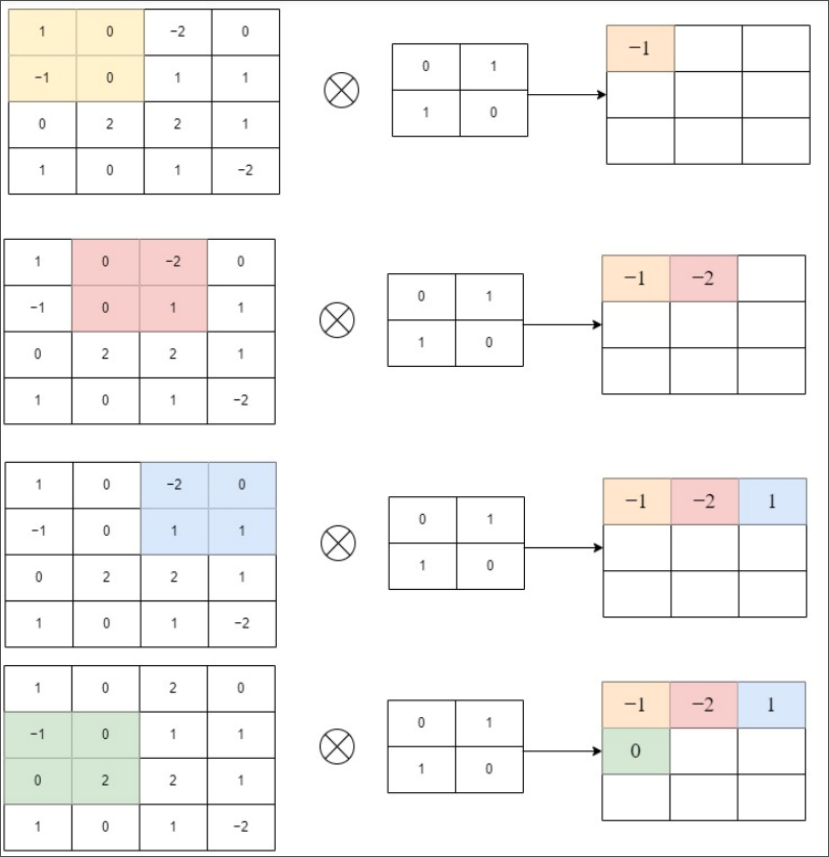
\includegraphics[width=0.4\textwidth]{informatica/ejemplo_capa_convolucional}
    \caption{Ejemplo gráfico de una convolución sobre una imagen (tensor de dimensiones $4 \times 4$). Estamos usando una convolución de tamaño $2 \times 2$, \textit{stride} = 1 y no usamos \textit{padding} (usamos otra política, que consiste en ajustar la convolución para que no se salga de la imagen). Imagen extraída de \cite{informatica:paper_definicion_cnn}.}
\end{figure}

Algunas características centrales de esta operación son:

\begin{itemize}
    \item \textbf{Coeficientes compartidos}: los coeficientes del operador son independientes de la posición en la que nos encontremos. Si nuestra convolución detecta un patrón, dicha detección debe ser independiente de la posición en la que se encuentre dicho patrón.
    \item \textbf{Localidad}: el operador toma información de vecindarios de elementos. Esto es relevante por la estructura local que hemos comentado de las imágenes o de los grafos.
\end{itemize}

\subsection{Bloques convolucionales y \textit{feature maps}}

Como hemos introducido previamente, una convolución puede operar sobre una imagen, que puede representarse como un tensor de dimensiones $ancho \times alto \times canales$, y producir un tensor de salida de dimensiones $ancho'  \times alto' \times 1$.

Lo normal en una capa de una red convolucional es aplicar más de una convolución. Por ejemplo, aplicar 8 convoluciones sobre la imagen de entrada. Esto produce 8 tensores de salida de dimensiones $ancho' \times alto' \times 1$, que se juntan en un tensor de dimensiones $ancho' \times alto' \times 8$. Cada una de las salidas del bloque convolucional se denomina en el ámbito del aprendizaje automático como \textit{feature map} o mapa de características.

Por tanto, un bloque convolucional toma un tensor de dimensiones $ancho \times alto \times profundidad$ y produce otro tensor de dimensiones $ancho' \times alto' \times profundidad'$. En el caso de ser el primer bloque, la $profundidad$ se corresponde con el número de canales de la imagen (por ejemplo, 3 en el caso de trabajar con imágenes \textit{RGB}). En el caso de bloques intermedios, la $profundidad$ se corresponde con el número de \textit{feature maps} que la anterior capa produce. Y eligiendo cuántos \textit{feature maps} producimos en un bloque concreto (lo que es lo mismo, cuántas convoluciones aplicamos), escogemos el valor de $profundidad'$.

Finalmente, los parámetros que definen una capa convolucional son:

\begin{itemize}
    \item Los parámetros de la operación de convolución que hemos comentado previamente
    \item \textit{Depth}: cuántos filtros convolucionales se aplican en esta capa. Esto determina el número de \textit{feature maps} producidas
\end{itemize}

\subsection{\textit{Pooling}}

El propósito de este tipo de capas es resumir la información de la imagen o del conjunto de mapas de activación para obtener datos de menor dimensionalidad. Hay varias formas de realizar esta operación, así que mencionamos algunas de las más usuales:

\begin{itemize}
    \item \textit{Gobal pooling}: tomamos todos los datos y los resumimos como uno solo. Algunas formas de hace esto son:
        \begin{itemize}
            \item Utilizando la media de todos los valores.
            \item Utilizando el producto de todos los valores, lo que se conoce como \textit{Global Product Pooling}.
        \end{itemize}
    \item \textit{Max Pooling}: aplicamos un filtro que recorre la imagen de la misma forma que una convolución. Pero en vez de aplicar cierta suma ponderada, toma el máximo de los valores que se están considerando en ese paso.
    \item \textit{Average Pooling}: igual que \textit{max pooling}, pero en vez de tomar el máximo, se toma la media de los valores considerados.
\end{itemize}

Por lo tanto, en el \textit{max pooling} y \textit{average pooling} tenemos que definir el tamaño de ventana, que determinará cuántos elementos se agregarán en cada paso. Todo esto queda explicado en la siguiente figura:

\begin{figure}[H]
    \centering
    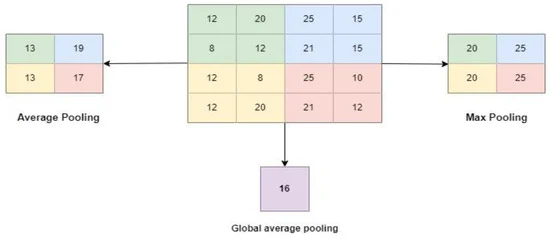
\includegraphics[width=0.6\textwidth]{informatica/ejemplo_pooling}
    \caption{Ejemplo gráfico de los tres tipos de \textit{pooling} que hemos comentado. Imagen extraída de \cite{informatica:paper_definicion_cnn}}
\end{figure}
\todo{Solucionar imagen de mala calidad}

Esta capa ayuda a que la red sea más ligera, pues al reducir la dimensionalidad de los datos, reduce el número de parámetros que necesitamos ajustar. A partir de la experimentación se piensa que además ayuda a introducir cierta invarianza frente a traslaciones.

\subsubsection{Capa totalmente conectada} \label{subsubs:capa_totalmente_conectada}

También conocidas como \textit{linear dense layers} o capas lineales densas. Estas capas toman un vector de valores de entrada, realizan una combinación lineal de sus valores, y en la mayoría de casos, aplican una función no lineal a la salida. Por lo tanto, una capa totalmente conectada viene dada por:

\begin{itemize}
    \item La dimensión de los vectores que puede procesar, $N$
    \item Los pesos de la combinación lineal que realiza sobre las entradas, $w_1, \ldots, w_N$
    \item La función de activación no lineal, si es que la hubiera, $\sigma: \R \to \R$
\end{itemize}

Por lo tanto, el funcionamiento de una capa lineal densa se resume en:

\begin{equation}
    (x_1, \ldots, x_N) \to \sigma(\sum_{i = 1}^{N} w_i \; x_i)
\end{equation}

Estamos suponiendo que queramos que la salida de la capa sea un único valor escalar. Sin embargo, podemos generalizar esta operación para que la salida sea un vector de dimensión $S$. Para ello, basta considerar:

\begin{equation}
      f_\theta(\nv{x}) = \sigma(\nv{x}^T \nv{w} + b)
\end{equation}

donde $\theta = (\nv{w}, b)$ con $\nv{w} \in \R^s$, $b \in \R$.

Estas capas se suelen poner al final de las redes convolucionales, para realizar la predicción final. Toman las características jerárquicas que las convoluciones extraen y las combinan para resolver la tarea planteada. Para ello, debemos vectorizar el tensor de entrada, pero esto es una operación trivial.
